% !TEX root = paper.tex

\section {Results}
\label{sec:results}

\begin{figure}[!hbt]
	\centering
	\subfigure{ 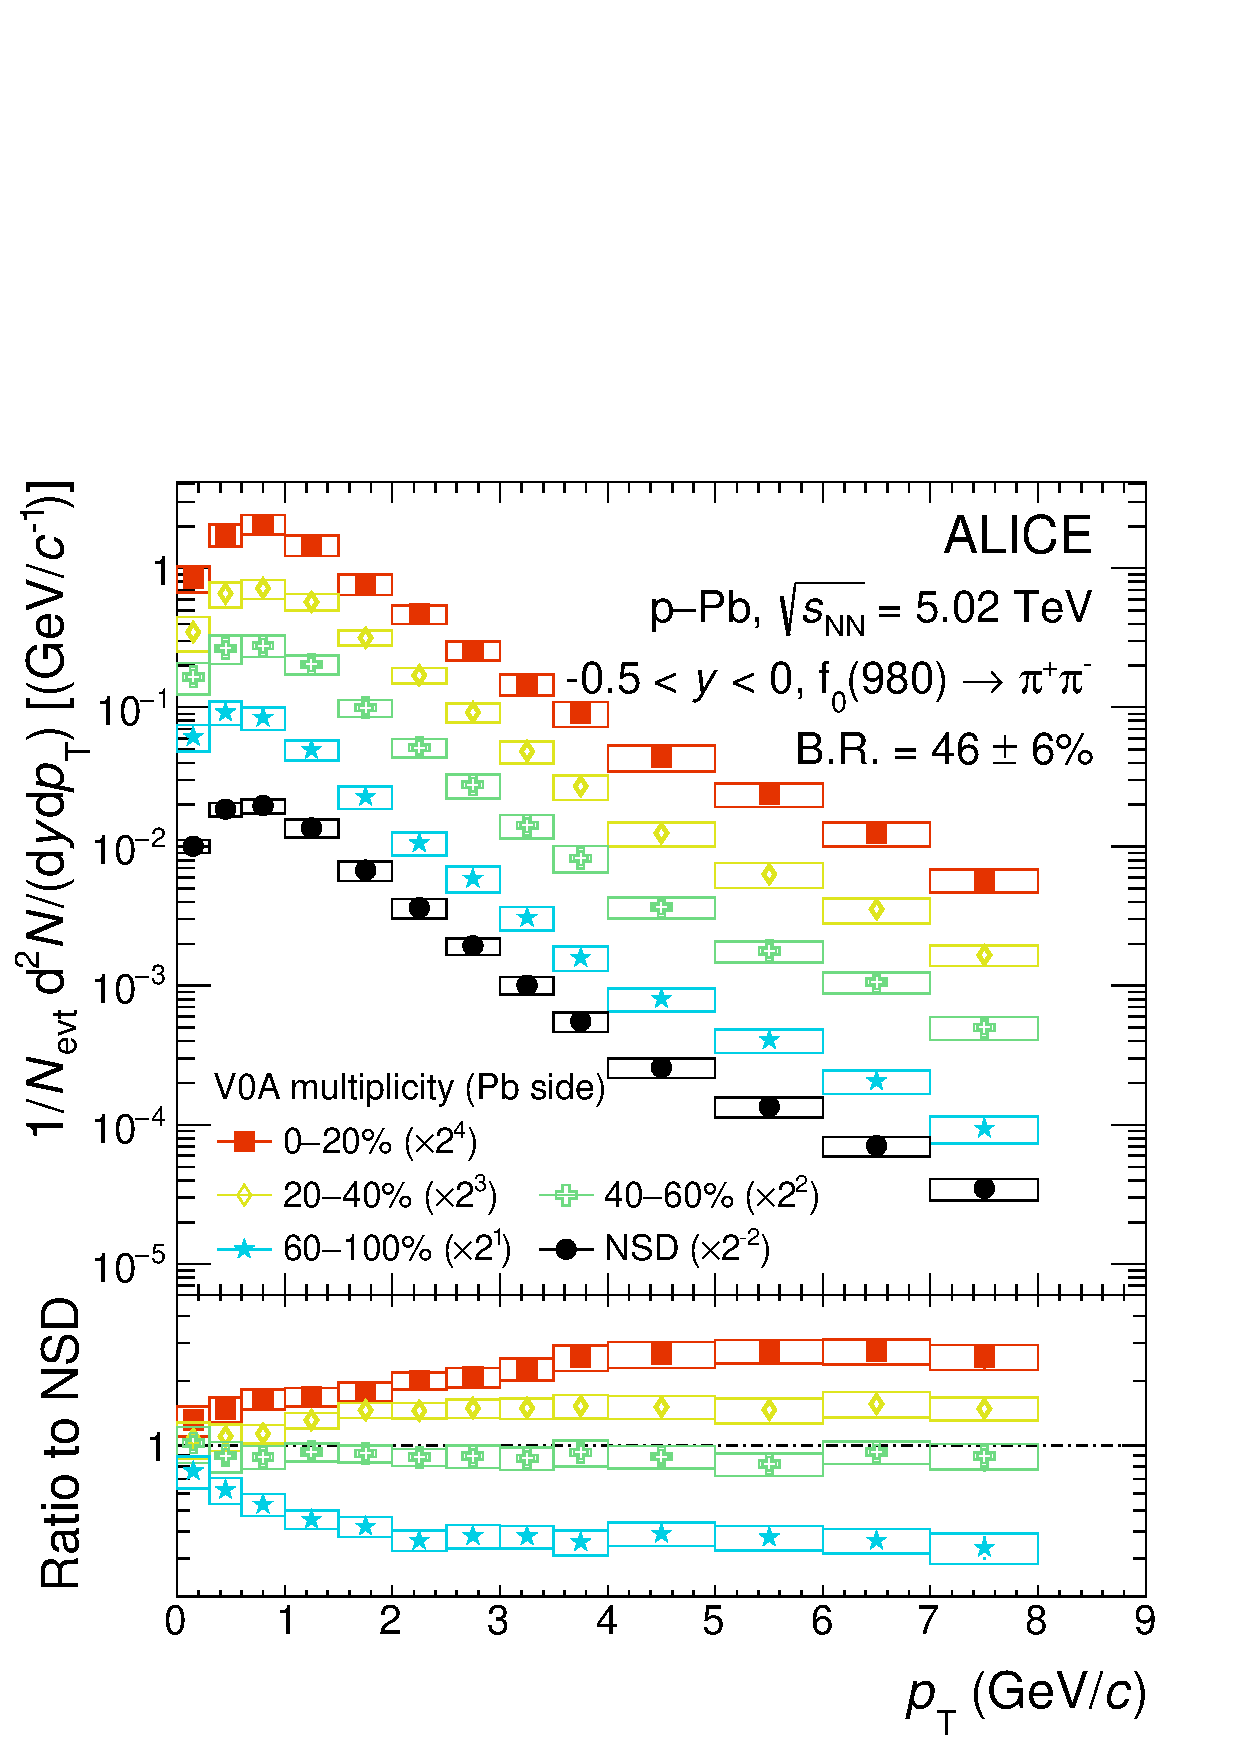
\includegraphics[width=0.6 \textwidth]{figures/Fig2_pt_all.pdf} }
	\caption{ Transverse momentum spectra of \fzero~in p--Pb collisions at \snn~=~5.02~TeV for different multiplicity classes, which are scaled for visibility. Statistical and systematic uncertainties are shown as error bars and boxes, respectively. The lower panel shows the ratios of the specific spectra to the minimum-bias NSD spectrum. }
	\label{fig:pt}
\end{figure}

Figure~\ref{fig:pt} shows the $p_{\mathrm{T}}$ spectra of \fzero~in p--Pb collisions at \snn~=~5.02~TeV measured in the ragne of 0~$<p_{\mathrm{T}}<$~8~GeV/$c$ for different multiplicity classes. Each spectrum is scaled with the number denoted in the figure for visibility. The lower panel of Fig.~\ref{fig:pt} shows the ratios of each $p_{\mathrm{T}}$ spectrum to the minimum-bias $p_{\mathrm{T}}$ spectrum. Increasing mean $p_{\mathrm{T}}$ are observed with the increasing multiplicity.

\begin{figure}[!hbt]
	\centering
	\subfigure{ 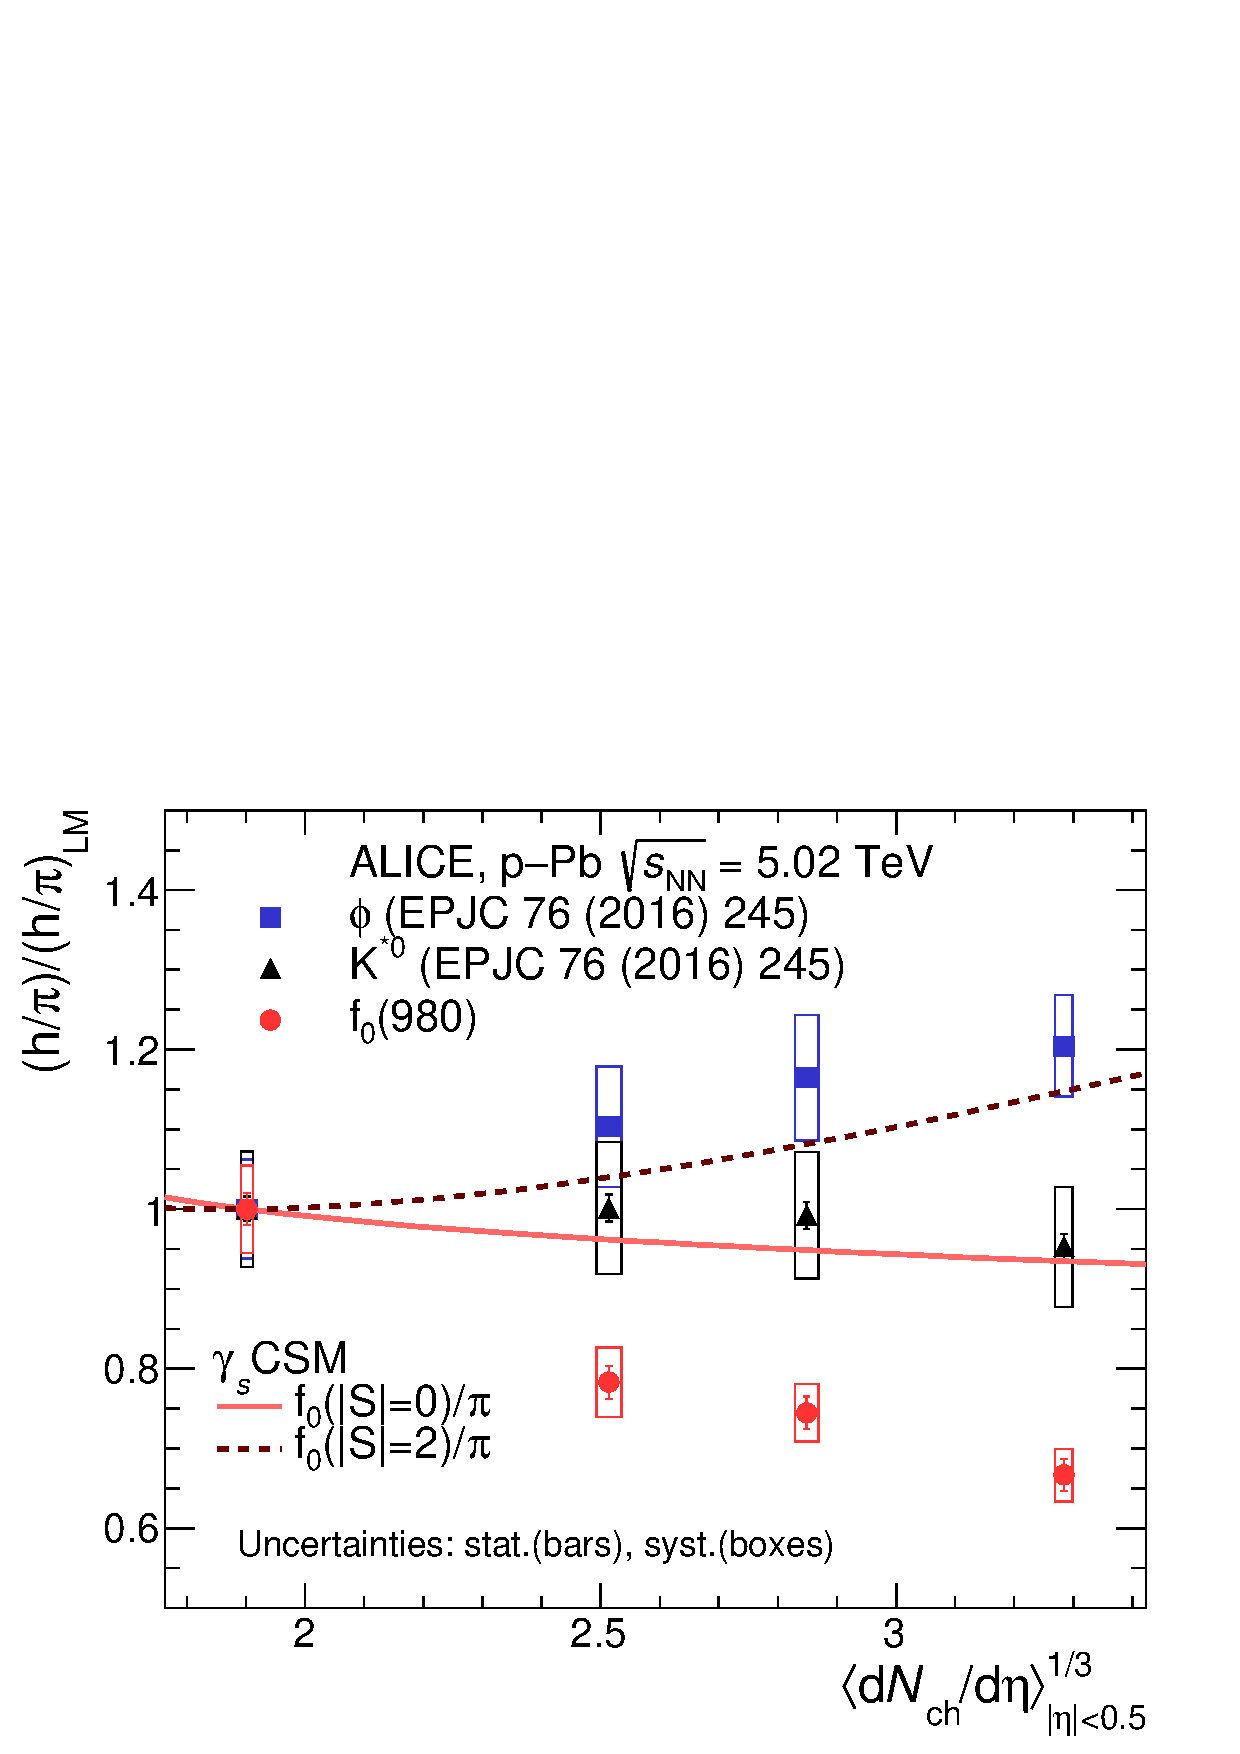
\includegraphics[width=0.6 \textwidth]{figures/Fig4_dr_pion_addCSM.pdf} }
	\caption{ Double ratio of $\phi$, $K^{*0}$(892), and \fzero~to $\pi$ as a function of charged-particle multiplicity. The ratios are divided by the ratio in low-multiplicity events to make the first point unity. Predictions from Canonical statistical model are represented with solid lines. }
	\label{fig:f0piAddCSM}
\end{figure}

Figure~\ref{fig:f0piAddCSM} shows the double ratio of different particles to charged pion yields as a function of multiplicity in p--Pb collisions at \snn~=~5.02~TeV. The ratio of $\phi$ to $\pi$ is increasing with multiplicity, which is observation of the strangeness enhancement~\cite{ALICE:2016fzo}. The ratio of $K^{*0}$ to $\pi$ is flat with multiplicity even $K^{*0}$ includes one strange quark. The flat trend is due to the two competing effects between the strangeness enhancement and rescattering effects, where the lifetime of $K^{*0}$ is 4.2~fm/$c$~\cite{ParticleDataGroup:2020ssz} and short enough to experience rescattering effects. The ratio of \fzero~to $\pi$ is decreasing with multiplicity because of short lifetime of \fzero~, which suggests that \fzero~experiences rescattering effects. Predictions of the ratio of \fzero~to $\pi$ are shown in lines for different hidden strangeness assumptions, zero and two, for \fzero~by Canonical Statistical Model (CSM)~\cite{Vovchenko:2019kes}. CSM with two hidden strangeness estimates the ratio to be increasing, which is opposite to the experimental result. Furthermore, CSM with zero hidden strangeness estimates the ratio to be flat, which either overestimates the data. This is mainly due to that CSM does not consider rescattering effects, and \fzero~yields would be overestimated.  

\begin{figure}[!hbt]
	\centering
	\subfigure{ 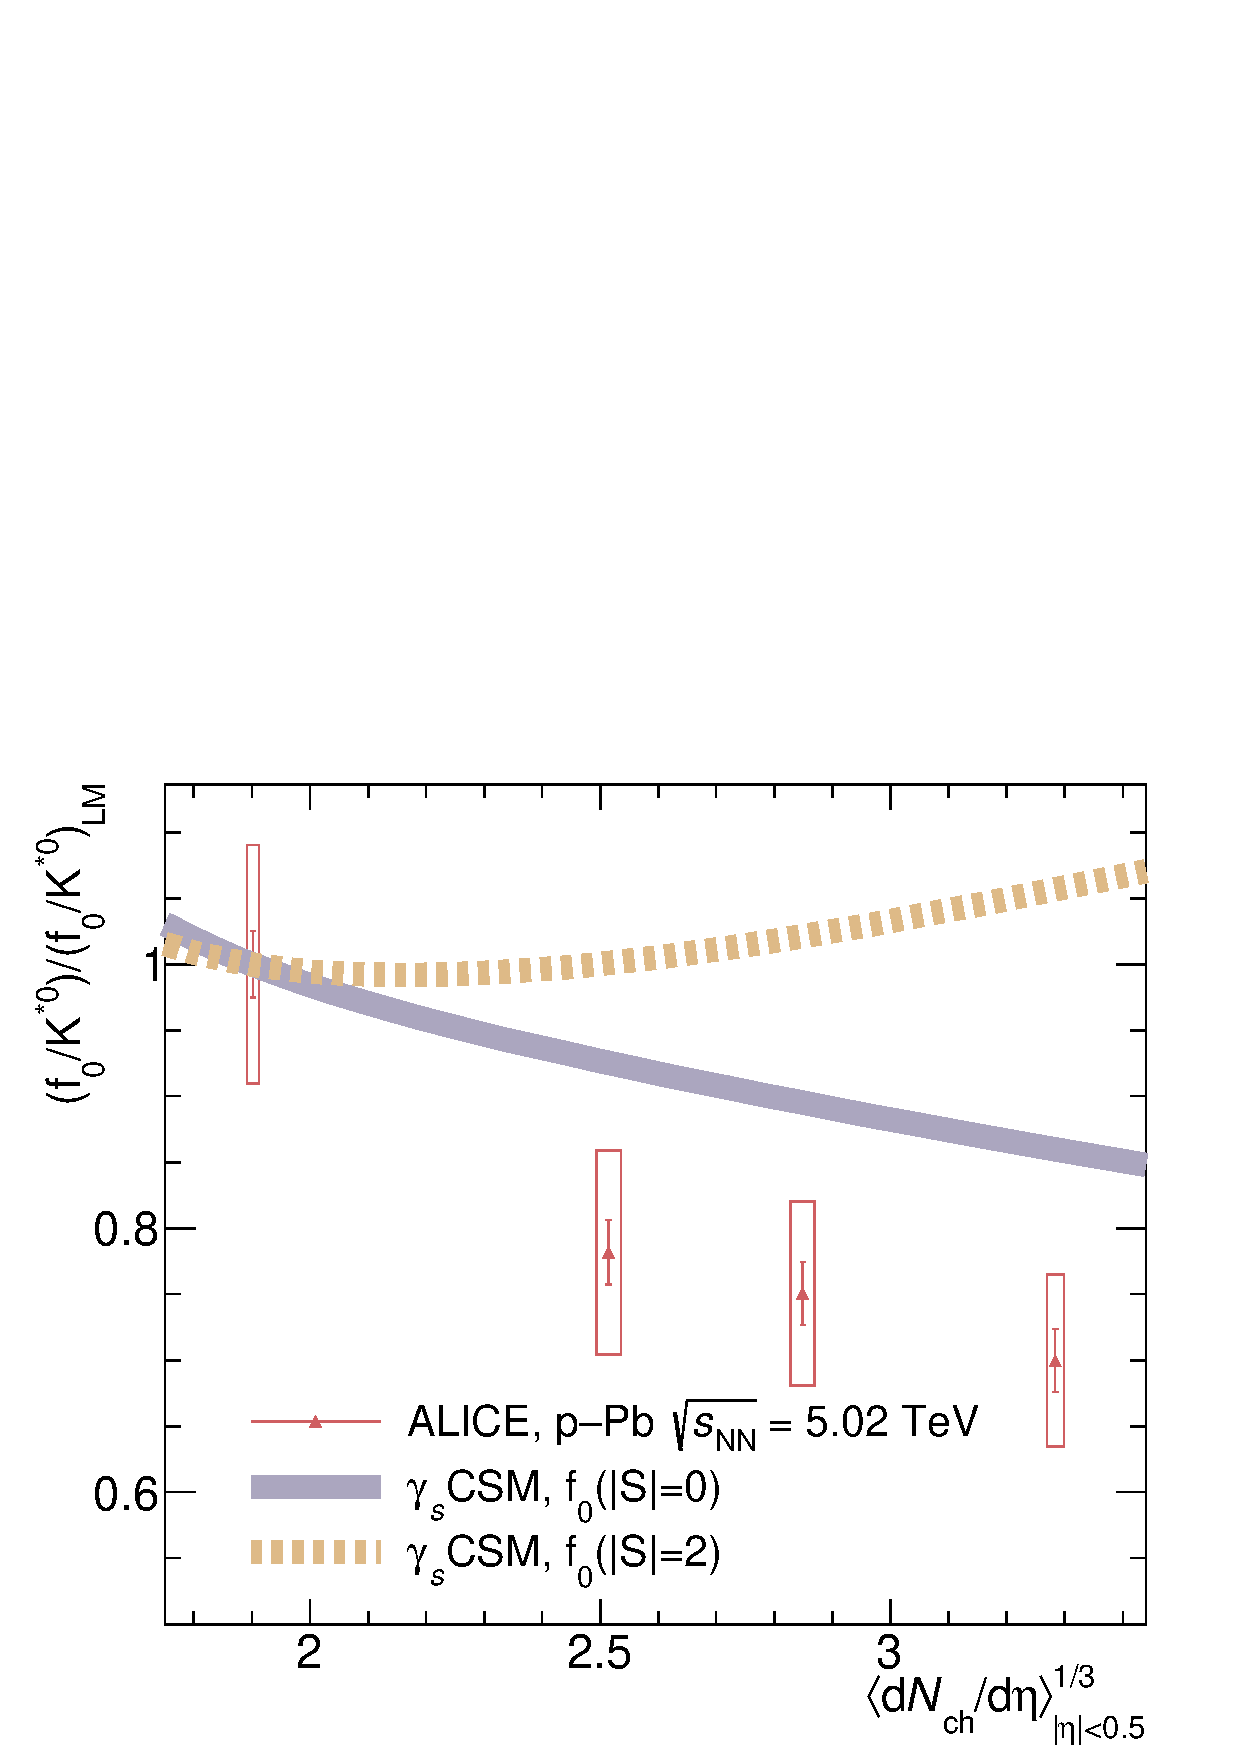
\includegraphics[width=0.6 \textwidth]{figures/Fig4_dr_kstar_addCSM.pdf} }
	\caption{ Double ratio of \fzero~to $K^{*0}$ yields as a function of charged-particle multiplicity. The ratios are divided by the ratio in low-multiplicity events to make the first point unity. Predictions from Canonical statistical model are represented with solid lines. }
	\label{fig:f0KSAddCSM}
\end{figure}

Figure~\ref{fig:f0KSAddCSM} shows the double ratio of \fzero~to $K^{*0}$ yields as a function of charged-particle multiplicity in p--Pb collisions at \snn~=~5.02~TeV and predictions from CSM with different hidden strangeness assumptions. The ratio is decreasing with multiplicity, and this trend is qualitatively described with the zero hidden strangeness assumption. Because the lifetimes of \fzero~and $K^{*0}$ are comparable each other, rescattering effects would be not much different. Thus, the decreasing trend of the ratio is rarely attributed to rescattering effects. CSM prediction with two hidden strangeness assumption is mildly increasing with multiplicity, which is also opposite trend to the experimental result. Therefore, decreasing trend of the ratio of \fzero~to $K^{*0}$ suggests no strange quark in \fzero.

\begin{figure}[!hbt]
	\centering
	\subfigure{ 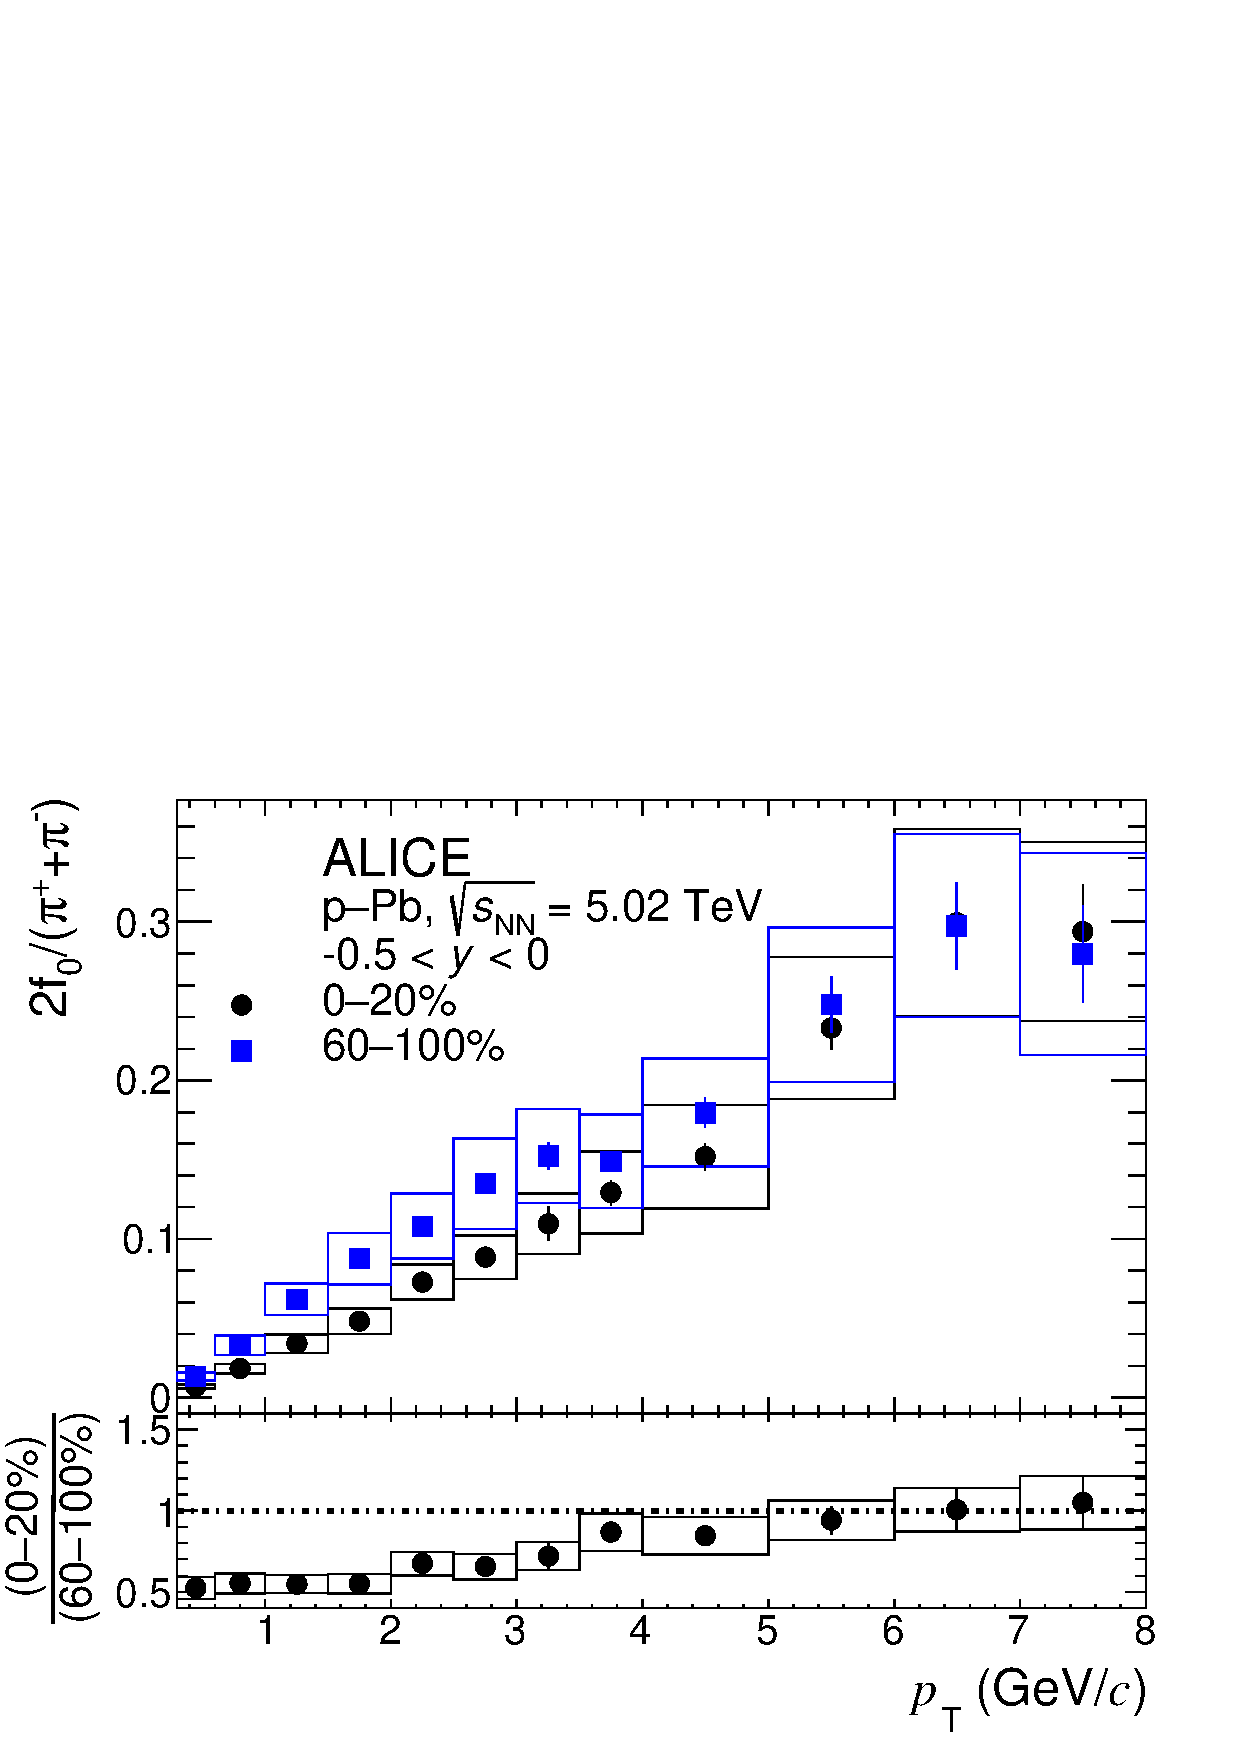
\includegraphics[width=0.6 \textwidth]{figures/Fig5_DR_pt_pion.pdf} }
	\caption{ Particle yield ratio of \fzero~to $\pi$ as a function of $p_{\rm{T}}$ in high-multiplicity (circles) and low-multiplicity (triangles) p--Pb collisions at \snn~5.02~TeV. The lower panel shows the double ratio of high-multiplicity to low-multiplicity \fzero/$\pi$. }
	\label{fig:f0piPt}
\end{figure}

Figure~\ref{fig:f0piPt} shows $p_{\mathrm{T}}$-differential particle yield ratio of \fzero~to $\pi$ in high-multiplicity and low-multiplicity p--Pb collisions at \snn~=~5.02~TeV. The ratios are consistent at high $p_{\mathrm{T}}>$~4~GeV/$c$ and getting different with decreasing $p_{\mathrm{T}}$. The lower panel shows the double ratio of high-multiplicity to low-multiplicity \fzero/$\pi$. There is strong suppression at low $p_{\mathrm{T}}$ and the suppression disappears as $p_{\mathrm{T}}$ increases. This is very similar $p_{\mathrm{T}}$ dependence with the $K^{*0}/K$~\cite{ALICE:2019etb}, where $K^{*0}/K$ is dominantly affected by rescattering effects.

\begin{figure}[!hbt]
	\centering
	\subfigure{ 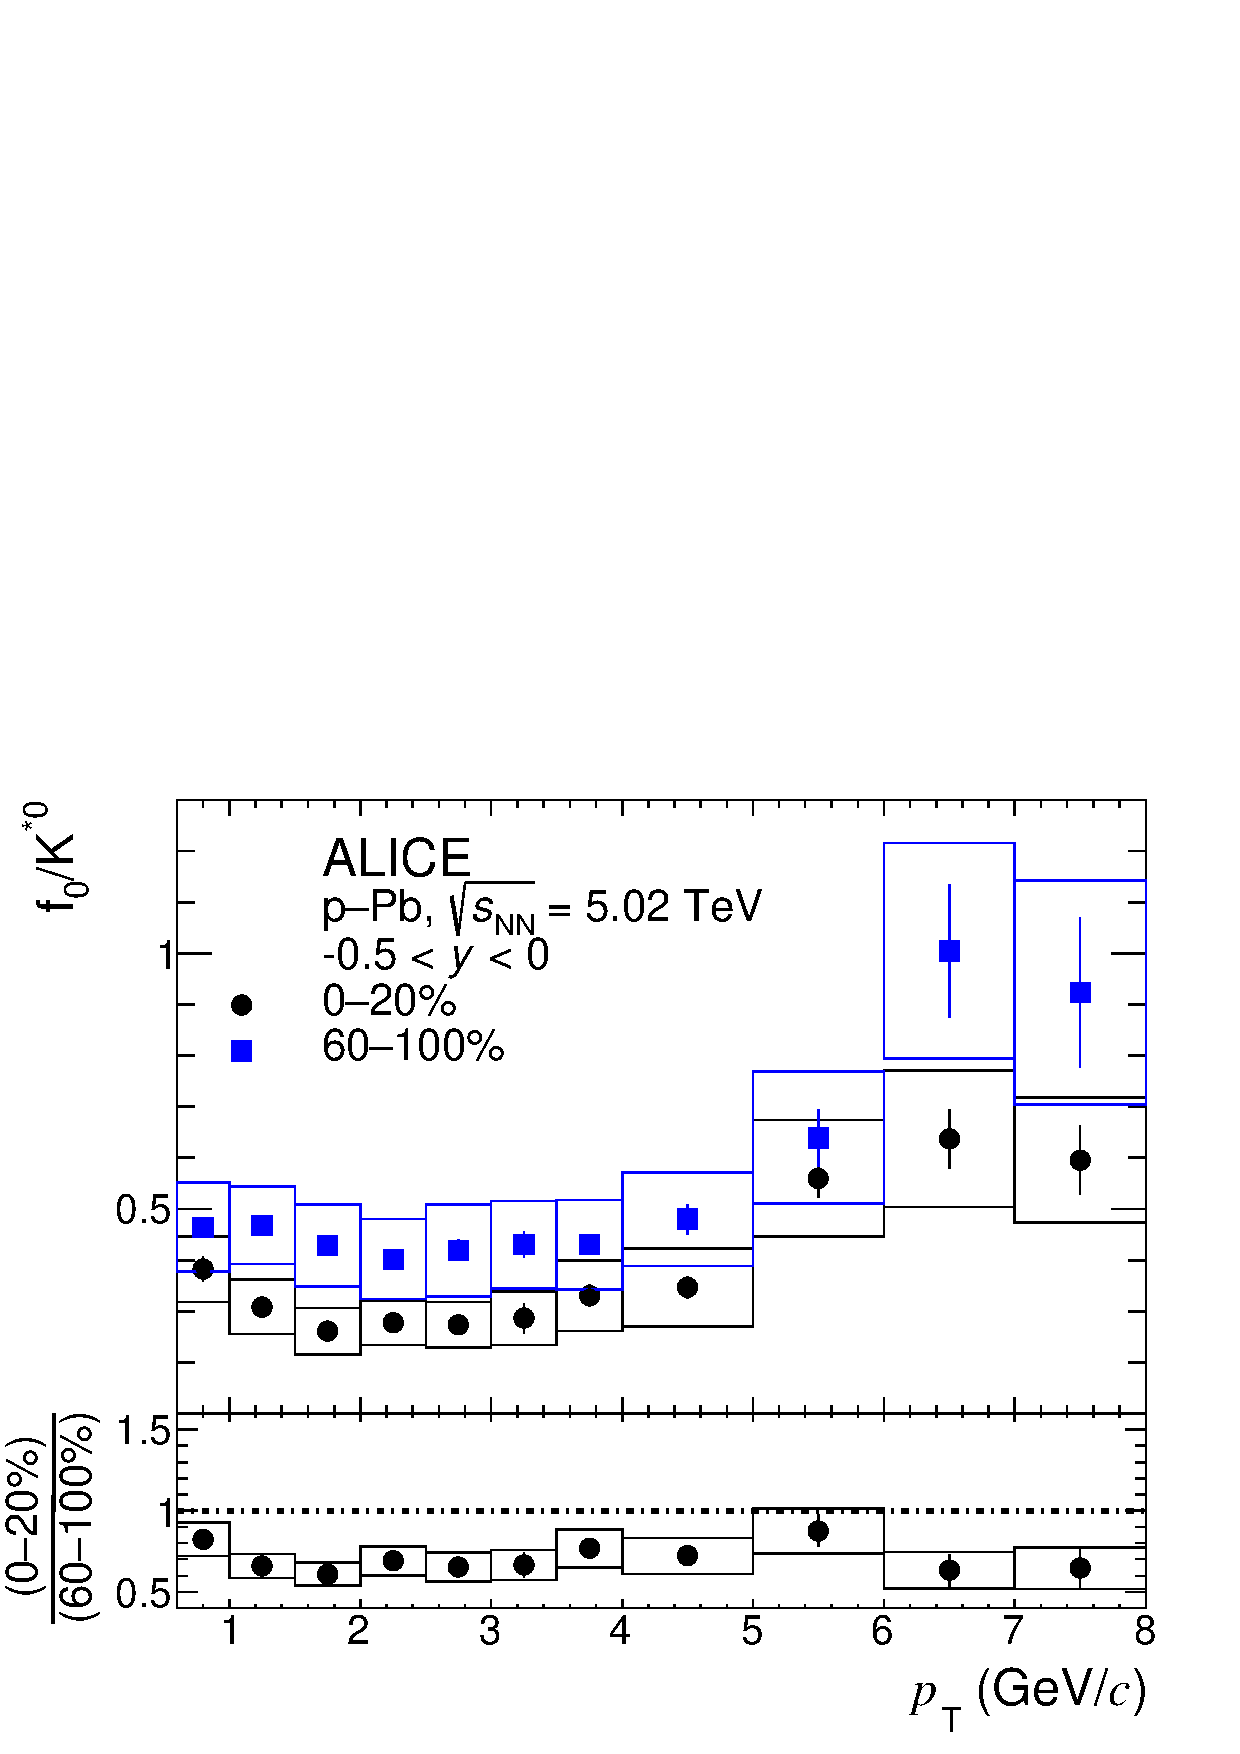
\includegraphics[width=0.6 \textwidth]{figures/Fig6_DR_pt_kstar.pdf} }
	\caption{ Particle yield ratio of \fzero~to $K^{*0}$(892) as a function of $p_{\rm{T}}$ in high-multiplicity (circles) and low-multiplicity (triangles) p--Pb collisions at \snn~5.02~TeV. The lower panel shows the double ratio of high-multiplicity to low-multiplicity \fzero/$K^{*0}$(892).  }
	\label{fig:f0KsPt}
\end{figure}

Figure~\ref{fig:f0KsPt} shows $p_{\mathrm{T}}$-differential particle yield ratio of \fzero~to $K^{*0}$ in high-multiplicity and low-multiplicity p--Pb collisions at \snn~=~5.02~TeV. The ratio from high-multiplicity events is suppressed in the entire $p_{\mathrm{T}}$ range, which is significantly different from the $p_{\mathrm{T}}$ dependence of $K^{*0}/K$ or \fzero/$\pi$. This would be explained with a mechanism rather than rescattering effects because the suppression for \fzero~exists not only at low $p_{\mathrm{T}}$ but also at high $p_{\mathrm{T}}$. This is, in opposite way, result from enhancement of $K^{*0}$ yield compared to \fzero~yield as $K^{*0}$ includes one strange quark.

\begin{figure}[!hbt]
	\centering
	\subfigure{ 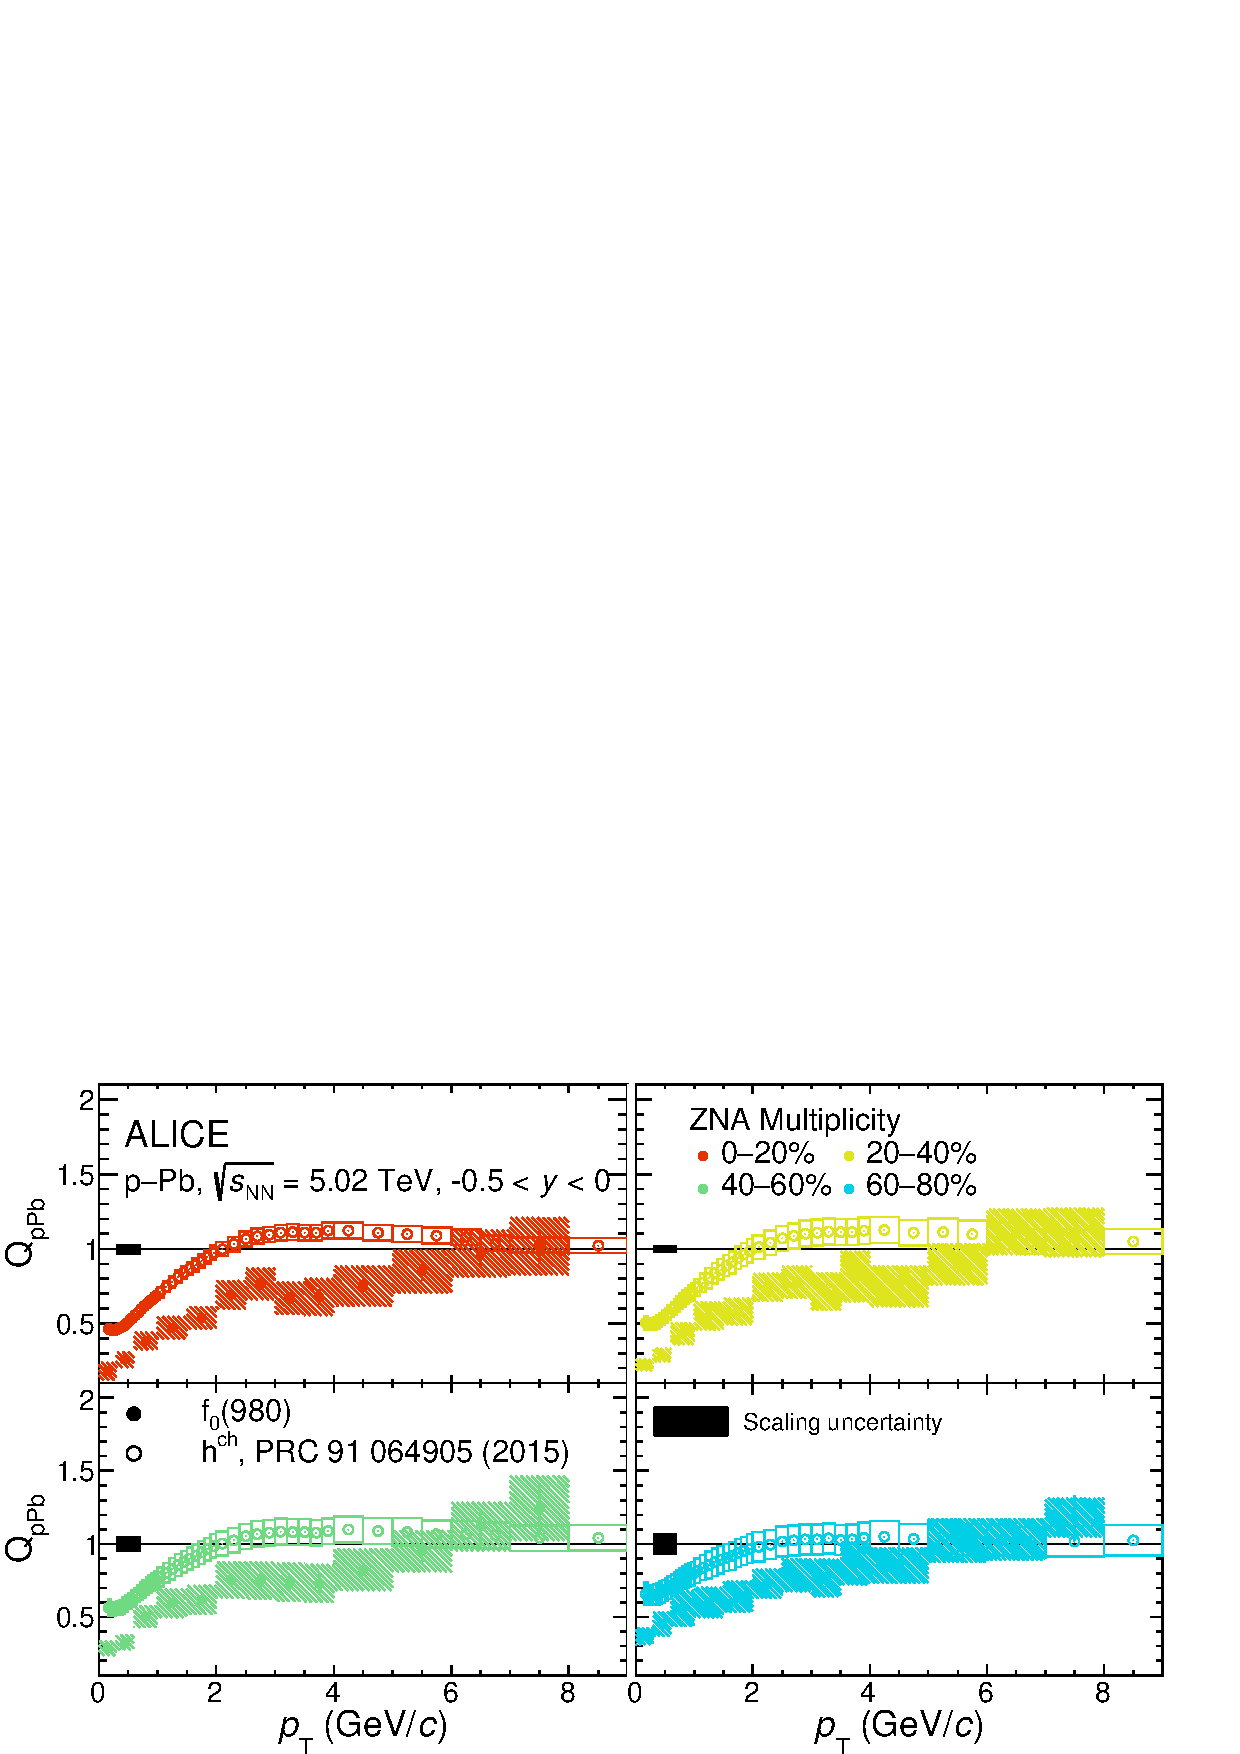
\includegraphics[width=0.8 \textwidth]{figures/Fig7_QpPb.pdf} }
	\caption{ Nuclear modification factor ($Q_{\rm{pPb}}$) of \fzero~as a function of $p_{\rm{T}}$ in p--Pb collisions at \snn~5.02~TeV for different multiplicity classes. Statistical and systematic uncertainties are shown as error bars and boxes, respectively. Open boxes around $p_{\rm{T}}$~=~0.5~GeV/$c$ represent the binary collision scaling uncertainties. The $Q_{\rm{pPb}}$ of \fzero~is compared with \fzero~of charged hadrons. }
	\label{fig:QpPb}
\end{figure}

Figure~\ref{fig:QpPb} shows the nuclear modification factor ($Q_{\rm{pPb}}$) of \fzero~in p--Pb collisions at \snn~=~5.02~TeV for different multiplicity classes. There is difference of $Q_{\rm{pPb}}$ between charged hadrons and \fzero~at low $p_{\mathrm{T}}$, and the difference is getting larger as the multiplicity class increases. On the other hand, there is no difference between charged hadrons $Q_{\rm{pPb}}$ and \fzero~$Q_{\rm{pPb}}$ at high $p_{\mathrm{T}}$. Furthermore, \fzero~$Q_{\rm{pPb}}$ has no Cronin peak~\cite{Cronin:1974zm} at the intermediate $p_{\mathrm{T}}$ even in high-multiplicity events, while all baryons exhibit Cronin peak. No Cronin peak for \fzero~might suggest the number of constituent quarks of \fzero.